% \usepackage{amssymb}

\subsection*{Methodology}
Our project is based on the code from the work of \cite{Amirian_2019_CVPR_Workshops}. The research adopts the deep learning algorithm infoGAN. However Amirian's method only uses infoGAN to try to avoid mode collapsing(??), not for factors deduction.

Generative Adversarial Network(GAN) consists of two parts, Generator G and Discriminator D. The both parts are neural network. Discriminator is a classifier, it tries to discriminate the real samples and fake samples. Generator generates fake samples and send them to the discriminator. Generator's task is fooling the discriminator by generating samples that close to the real samples. Generator and Discriminator actually play a two players mini-max game with the value function\cite{goodfellow2014generative}:
\[\underset{G}{min}\underset{D}{max} = \mathbb{E}_{\mathbf{x}~p_{data}(\mathbf{x})}[logD(x)] + \mathbb{E}_{\mathbf{z}~p_{\mathbf{z}}(\mathbf{z})}[log(1 - D(G(\mathbf{z})))].\] Even though Generator can generate fake examples from the noise input \(\mathbf{z}\), this noise vector is entangled. In other words, we can not get any information from the input noise vector and can not control the out put of the Generator. On the contrary, infoGAN can deduce interpretable information from the input. Instead of single noise input, infoGAN accepts another input which is called latent code \(\mathbf{c}\). This latent code can be discrete or continuous. It also contains another neural network Q which is auxiliary network. The system structure is in \ref{infoGan}. This auxiliary network takes generated samples as input and outputs \(\mathbf{c'}\). \(\mathbf{c'}\)  should as close as to \( \mathbf{c}\). The min-max game of infoGAN becomes a game with the value function\cite{infogan}:
\[\underset{G,Q}{min}\underset{D}{max} \mathbf{V_{infoGAN}(D, G, Q)} = \mathbf{V_{D, G} - \lambda \mathbf{L_I(G,Q)}},\] where \(\mathbf{L_I(G,Q)}\) is the lower bound of the mutual information \(\mathbf{I(c;G(z,c))}\).
\begin{figure*}[h]
  \centering
  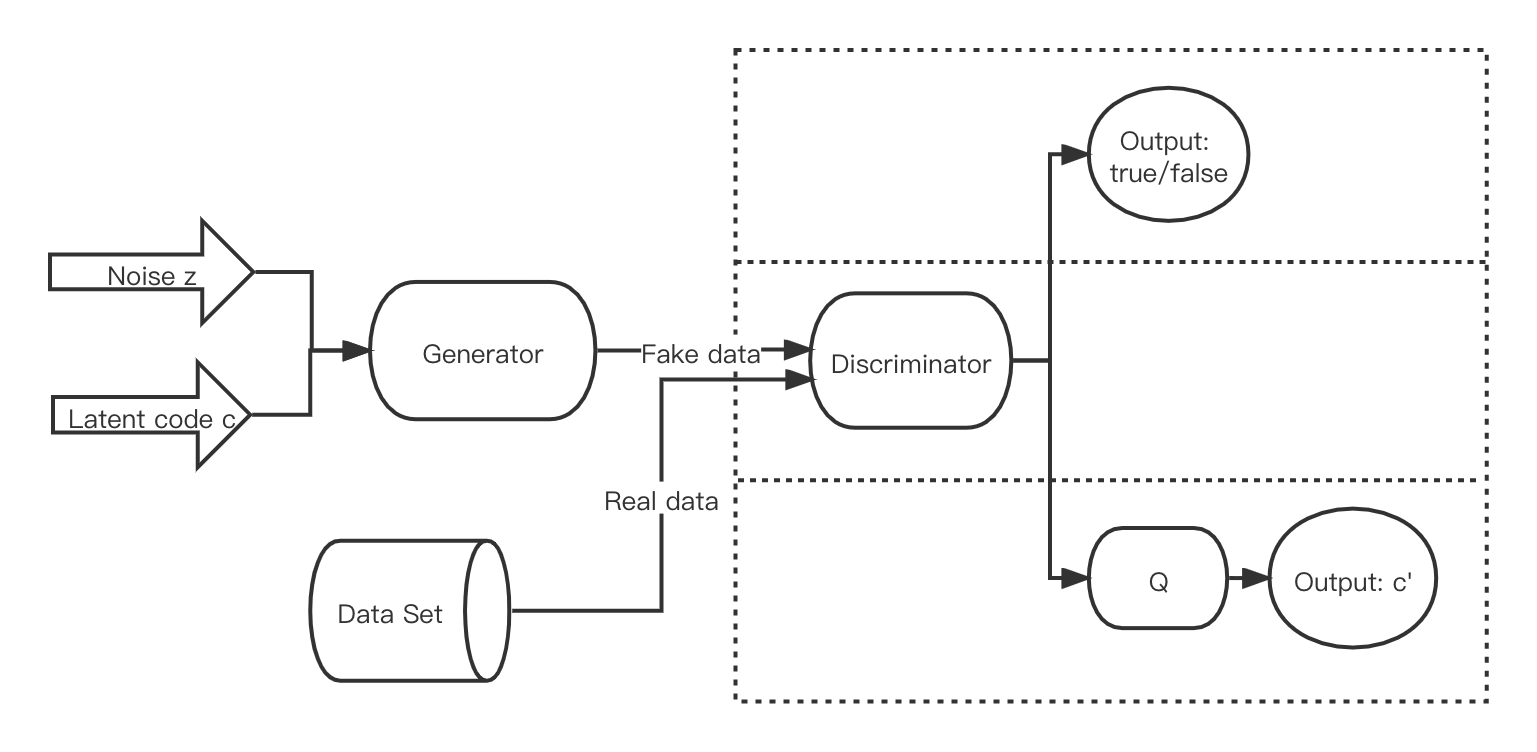
\includegraphics[width=\textwidth, height = 7cm]{figures/infoGAN.png}
  \caption{infoGAN Overview}{infoGAN consists of three parts, Generator G, Discriminator D and auxiliary network Q. D and Q share the network, only their last layers are different.}
%   \Description{infoGAN consists of 3 parts, Generator G, Discriminator D and auxiliary network Q. D and Q share the network, only their last layers are different.}
  \label{infoGan}
\end{figure*}

Based on the training result of latent code \(\mathbf{c}\), and use the Generator to generate data and observe the characteristics of the data, we may deduce the information implied by \(\mathbf{c}\). The process of getting interpretable information from the input latent code is disentanglement.

In our project, we add